\subsection{Data Preprocessing}

We separately tested the effects of three preprocessing techniques in 2.2 on the baseline model's performance.
In view of limited computational resources, we cannot fully optimize all the techniques,
so we only test a few hyperparameters for the techniques, especially for the filtering.

\subsubsection{Experiment Settings}
First, we applied a notch filter to remove power line interference at 50 Hz.
Upon investigating previous works in sEMG signal processing, we found that the frequency range of sEMG signals is primarily between 20 Hz and 150 Hz.
Therefore, we trained the model (with the notch filter already added) with a bandpass filter with a cutoff frequency of 20 Hz and 500 Hz or with another bandpass filter with a cutoff frequency of 20 Hz and 150 Hz.
We trained the three models and compared their performance at the end of Epoch 50.

For the adaptive Gaussian noise, we fixed the noise ratio  to 0.05, which is a relatively small value.
Because of time constraints, we did not test other values.

\subsubsection{Results}

\begin{figure}
    \centering
    % 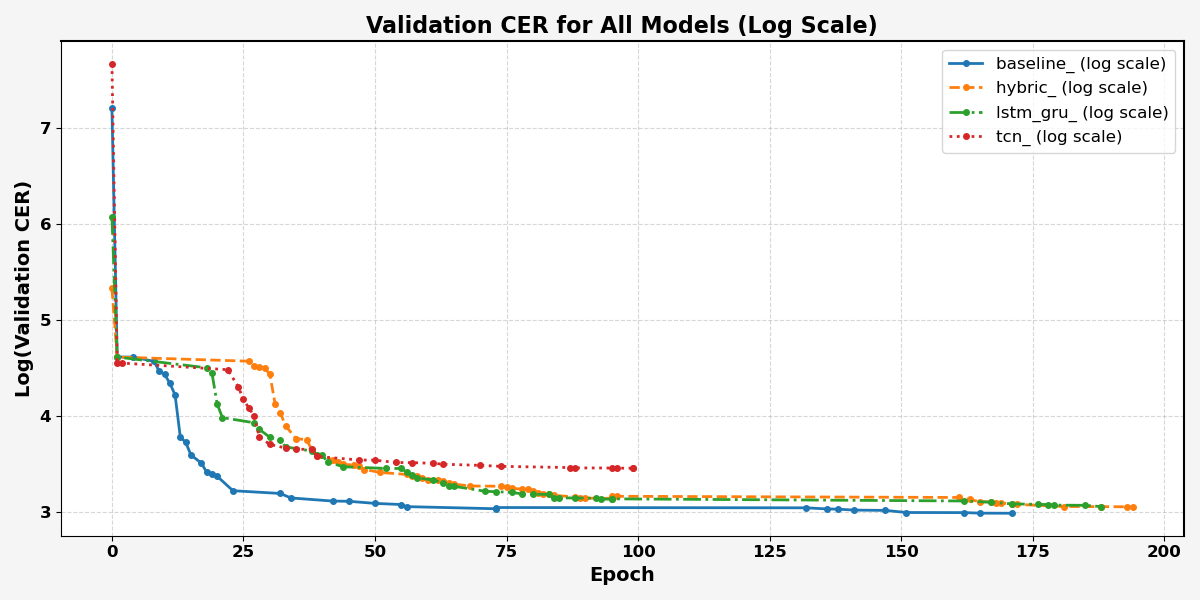
\includegraphics[width=0.8\textwidth]{figures/Val_cer.png}
    \caption{Comparison of the CER of the baseline model and the models with preprocessing techniques}
\end{figure}
  

As shown in , we found that the validation CER of model with the notch filter surpassed the baseline model by 8.2\% at the end of Epoch 50.
The model with adaptive Gaussian noise and the model with z-score normalization also achieved a CER of 22.13 and 22.37 respectively, 
which is quite close to the baseline model's CER of 20.98.
However, the model with the bandpass filters both performed poorly, while they had a very high CER at the beginning of training.

It is also worth noting that the models with any of the preprocessing techniques performed much better than the baseline model at the beginning of training, 
all of which had a CER that was 5 times lower than the baseline model.
This indicates that the preprocessing techniques can help the model converge faster.
The models with bandpass filters and z-score normalization especially performed well at the beginning of training.
